\chapter{Analysis of Survival Times} \index{general}{survival times}

When analyzing survival times, different problems come up than the ones discussed so far. One question is how to deal with subjects dropping out of a study. For example, assume that we test a new cancer drug. While some subjects die, others may believe that the new drug is not effective, and decide to drop out of the study before the study is finished.
A similar problem would be faced when we investigate how long a machine lasts before it breaks down. "Survival analysis"  is also used to analyze for example how long people subscribe to mailing lists (where the "death" corresponds to unsubscribing from a mailing list).

\section{Survival Distributions}

The Weibull distribution is the often used for modeling reliability data or survival data. Since it was first identified by Frechet (in 1927), but described in Detail by Weibull (in 1951), it is sometimes also found under the name Frechet distribution\index{general}{distributions!Frechet}.

In \lstinline{scipy.stats}, the Weibull distribution is available under the name \lstinline{weibull_min}, or equivalently \lstinline{frechet_r} for "Fréchet right".  The complementary \lstinline{weibull_max} (also called \lstinline{frechet_l} for "Fréchet left") is simply mirrored about the origin.

The Weibull distribution is characterized by a shape parameter, the Weibull Modulus $k$ (see also section \ref{sec:Weibull}). All \emph{Python}-distributions offer a convenient method \emph{fit}, which allow a quick fitting of the distribution parameters:

\lstinputlisting[label=py:WeibullDemo,caption=WeibullDemo.py, language=Python]{../Code3/WeibullDemo.py}

\section{Survival Probabilities}

For statistical analysis of survival data, Cam Davidson-Pilon has developed the \emph{Python} package \emph{lifelines}. It can be installed with

\begin{lstlisting}
  pip install lifelines
\end{lstlisting}

 A very extensive documentation, which also includes an introduction to survival analysis and survival regression modeling, is available under \url{http://lifelines.readthedocs.org/}.

\subsection{Censorship}\index{general}{censorship}

The difficulty of using data for survival analysis is that at the end of a study, many individuals may be still "alive". As an example let us consider a mailing list, whose subscribers fall into two subgroups. Group One quickly gets tired of the emails, and unsubscribes after three months. Group Two enjoys it, and typically subscribes for one and a half years. We perform a study which lasts one year, and want to investigate the average subscription duration:

\begin{figure}[H]
  \centering
  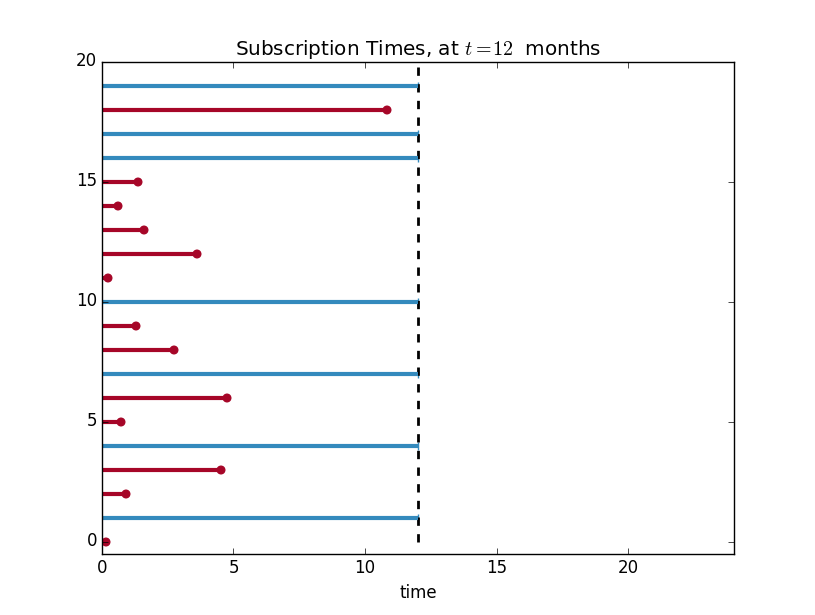
\includegraphics[width=0.75\textwidth]{../Images/lifelines.png}\\
  \caption{Dummy results from a study on the subscription behavior of a mailing list.}\label{fig:lifelines}
\end{figure}

\PyImg "lifelinesDemo.py" (p \pageref{py:lifelines}): Graphical representation of lifelines.
\index{python}{lifelinesDemo}

The red lines denote the subscription time of individuals where the dropout event has been observed, and the blue lines denote the subscription time of the right-censored\index{general}{right-censored data} individuals (dropouts have not been observed). If we are asked to estimate the average subscription time of our population, and we naively decided to not included the right-censored individuals, it is clear that we would be severely underestimating the true average subscription time.

A similar, further problem occurs if some subject increase their privacy-setting in the middle of the study, i.e. they forbid us to monitor them before the study is over. Also these data are right-censored data.

\subsection{Kaplan-Meier survival curve} \index{general}{Kaplan-Meier survival curve}

A clever way to deal with these problems is the description of such data with the Kaplan-Meier curve, described in detail in \cite{altman99}. First, the time is subdivided into small periods. Then the likelihood is calculated that a subject survives a given period. The survival probability is given by

\begin{equation}
  p_k = p_{k-1} * \frac{r_k-f_k}{r_k}
\end{equation}

where $p_k$ is the probability to survive period $k$; $r_k$ is the number of subjects still at risk (i.e. still being followed up) immediately before the $k^{th}$ day, and $f_k$ is the number of observed failures on the day $k$. The curve describing the resulting survival probability is called Life Table, Survival Curve, or Kaplan-Meier Curve (see Figure \ref{fig:SurvivalCurve}).

The following data show the genotypes and number of days survived in Drosophila. Since we work with flies, we don't need to worry about left-censoring. We know the birth date of all flies. We do have issues with accidentally killing some or if some escape. These would be right-censored as we do not actually observe their death due to "natural" causes. ( miR-137 is a short non-coding RNA molecule that functions to regulate the expression levels of other genes.)

\lstinputlisting[label=py:lifelinesSurvival,caption=lifelinesSurvival.py, language=Python]{../Code3/lifelinesSurvival.py}


\begin{figure}
  \centering
  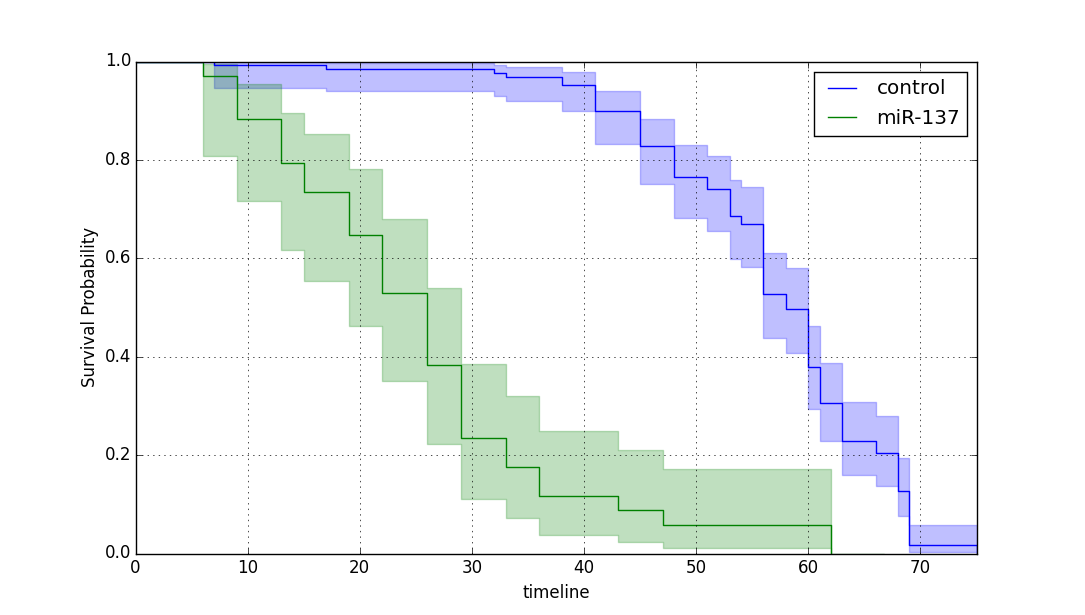
\includegraphics[width=0.75\textwidth]{../Images/lifelines_survival.png}\\
  \caption{Survival Probability of two groups of Drosophila flies. The shaded areas indicate the 95\% confidence intervals.}\label{fig:SurvivalCurve}
\end{figure}

Note that the survival curve changes only when a "failure" occurs, i.e. when a subject dies. \emph{Censored} entries, describing either when a subject drops out of the study or when the study finishes, are taken into consideration at the "failure" times, but otherwise do not affect the survival curve.

\section{Comparing Survival Curves in Two Groups} \index{general}{test!logrank}

The most common test for comparing independent groups of survival times is the \emph{logrank test}. This test is a non-parametric hypothesis test, testing the probability that both groups come from the same underlying population. To explore the effect of different variables on survival, more advanced methods are required. For example, the Cox Regression model\index{general}{Cox regression model}, also called Cox Proportional Hazards model\index{general}{Cox proportional hazards model} introduced by Cox in 1972 is used widely when it is desired to investigate several variables at the same time.

These tests, as well as other models for the analysis of survival data, are available in the \emph{lifelines} package.